\documentclass[11pt]{article}
\usepackage[utf8]{inputenc}
\usepackage{float}

\usepackage{geometry}
 \geometry{
     a4paper,
     left=25mm,
     top=25mm,
     right=25mm,
     bottom=30mm
 }

%% for colors
\usepackage{xcolor} % must be loaded erly
%% Define your custom colors
\definecolor{myblue}{HTML}{648FFF}
\definecolor{mypurple}{HTML}{775EF0}
\definecolor{myred}{HTML}{DD2680}
\definecolor{myorange}{HTML}{FE6100}
\definecolor{myyellow}{HTML}{FFB001}
% Create a new command for the colors
\newcommand{\blue}[1]{\textcolor{myblue}{#1}}
\newcommand{\purple}[1]{\textcolor{mypurple}{#1}}
\newcommand{\red}[1]{\textcolor{myred}{#1}}
\newcommand{\orange}[1]{\textcolor{myorange}{#1}}
\newcommand{\yellow}[1]{\textcolor{myyellow}{#1}}
 
%% for tables
% for dashed and dotted lines
\usepackage{tabularray}
\usepackage{booktabs} % For better hlines in tables
% used to add notes to figures and table with fnote command
\newcommand\fnote[1]{\captionsetup{font=small}\caption*{#1}}
% for tables with cells spanning several rows
\usepackage{multirow}
\usepackage{makecell}
%% for grafics and figures
\usepackage{graphicx}
\usepackage{svg}  % to use .svg
\usepackage{tikz}
\usetikzlibrary{shapes,positioning,arrows,arrows.meta,fit, backgrounds}

%% for flexible list items
\usepackage{enumitem}

%% math 
\usepackage{amsmath}
\usepackage{amsthm}
\usepackage{mathtools} 
\usepackage{verbatim} 

%% format of captions and footnotes
\usepackage[font=small,labelfont=bf]{caption}
% flushing left of footnotes
\usepackage[hang,flushmargin]{footmisc}

%% links and urls
\usepackage[hidelinks]{hyperref}
\hypersetup{
    colorlinks=false,
    linkcolor=black,
    filecolor=magenta,      
    urlcolor=blue,
    citecolor=blue,
}
\urlstyle{same}

%% clever referencing and citing rule
\usepackage{cleveref}
\usepackage[sort, numbers]{natbib}
\usepackage{appendix}

%% new setting for \paragraph
\newcommand{\myparagraph}[1]{\paragraph{#1}\mbox{}\\}

%% format of inline code
\definecolor{codeColor}{gray}{0.85}
\usepackage{tcolorbox}
\newtcbox{\ilc}{on line, boxrule=0pt, boxsep=0pt, bottom = 0pt, left=0pt, right =0pt, top = 0pt, arc = 0pt, colback=white, colframe = white, fontupper={\small \ttfamily}}

%% for code snippets
\usepackage{listings}

\title{Text-Terminal: A UTF-8 Text Editor for the Linux Shell}

\author{\\ \\
Project Report\\
Operating Systems Lecture Spring Semester 2025 \\ \\ \\ \\
University of Basel \\
Faculty of Science \\
Department of Mathematics and Computer Science \\ \\ \\ \\
Heinrich Ahrend \\ 
Yorik Metzger \\
Jorn Riedel \\
Shura V. Ruben \\ \\ \\ \\}
\date{June DD, 2025 \vfill 
\includegraphics{resources/logo.jpg}} % TODO: Update for hand-in date

\begin{document}
    \maketitle
    \thispagestyle{empty}

    \clearpage
    \pagestyle{empty}
    \tableofcontents
    \clearpage    
    \pagestyle{plain}
    \setcounter{page}{1} % Start from page 1
    
    %% Here you add additional files for additional sections
    \section{Introduction}\label{sec:intro}

% Introduction: Introduce the problem you are trying to solve and the necessary context, motivate why solving this
% problem is important, highlight the significance of solving this problem. (What are you trying to do and why?)

Text editors are an essential tool that is quite often taken for granted since pretty much every single operating system has one included by default. Despite this, quite a lot of software engineering is required to develop a software product that is able to full fill the requirements posed by the tasks we need and wish to perform in our text editors. This is especially the case when features like word and line count should work well with very large files. \\
Since these aspects intrigued us and we wanted to try and develop our own solution from the ground up, we choose to develop a full text editor as our OS course project. More specifically we have opted to try and develop a plain text (file) editor, with good handling of large (even very large files), since this is one of the major weak points we identified with VS Code and other text editors. 
Additionally: 
\begin{itemize}
\item  it should support UTF-8 encoding since it is essential when writing a text in German and French.
\item it should be compatible with the three most common line break standards: \verb|\n| (Linux), \verb|\r\n| (Windows), \verb|\r| (Mac). 
\item the user interface should be a bit easier to use then pure keyboard text editors (e.g. vi/vim); it should allow to use the mouse for most important operations.
\item and finally the user interface should be responsive even when operating on large files.
\end{itemize}


    \section{Background}\label{sec:bg}
% Introduces relevant background knowledge to understand your work (e.g., existing algorithms,
% protocols, software, and technologies).

After researching possible approaches for storing the text, we settled on implementing our own \textit{piece table} data structure inspired by C. Crowley's discussion of text editor data structures \cite{crowley1998data}. The general idea of \textit{piece tables} is to store a sequence of \textit{piece descriptors}, which point to contiguous text spans in a buffer. By using a separate \textit{file buffer} for the file content and an append-only \textit{add buffer} for new content, the complexity of editing text is essentially reduced to updating this sequence of piece descriptors. Thus, by using memory mapping for the \textit{file buffer}, the size of the data structure only grows with the number of edits rather than with the file size. This makes \textit{piece tables} an excellent choice for out text editor intended to handle large files.
%GUI
\par
\smallskip
For building the text-based user interface we use ncursesw version 6 \cite{ncursesw}, because it is a library that supports various terminals. We specifically chose the wide character version of ncurses to support Unicode and international character sets (standard ncurses only has ASCII support).
\par
\smallskip
We also use xclip \cite{xclip} for our copy and paste functionality, which allows accessing the clipboard of the X11 windowing system. Although X11 is increasingly being replaced by Wayland on Linux systems, we have found that xclip remains compatible with most Wayland environments thanks to XWayland compatibility.
    \section{Methodology}\label{sec:meto}
% Conceptual explanation of implementation, configuration, and setup. (May use code snippets and
% screenshots to explain concepts, but not full code listings.)
After deciding on our project topic we fixed our software requirements in more concrete form. Having done so we identified that it would be most beneficial to divide our future code into front end and backed with the main interface being between graphical user interface (GUI) and text data structure. \\
The \verb|textStructure.h| header is the main interface connecting the GUI in \verb|main.c| and the actual text data structure implementation in \verb|textStructure.c|.
\begin{figure}[H]
\caption{Project Code Structure}
\noindent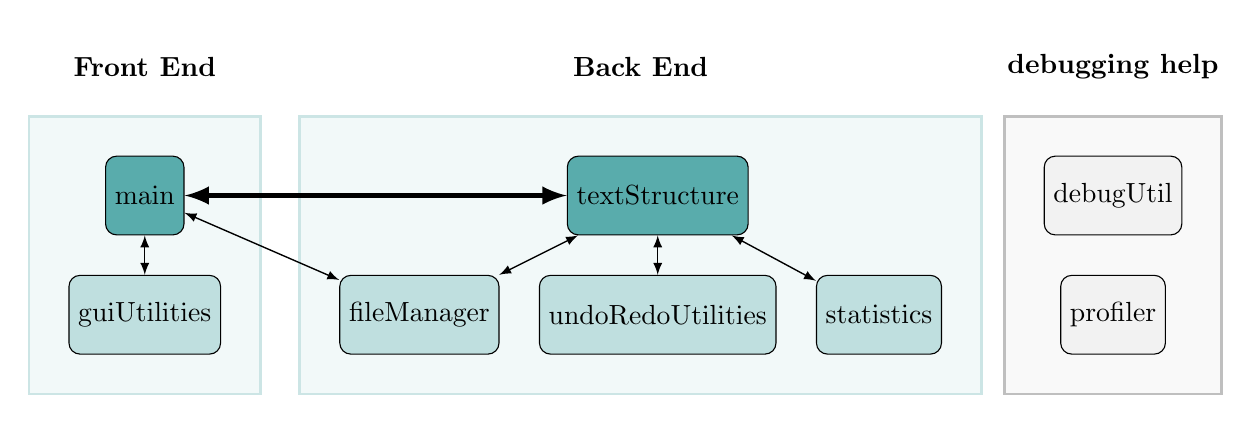
\begin{tikzpicture}[ 
    % Define node styles
    scale = 1,
    node distance = 0.5cm,
    minimum height = 1cm,
    imp/.style={rectangle, rounded corners, fill=teal!65, draw, align=center},
    file/.style={rectangle, rounded corners, fill=teal!25, draw, align=center},
    adj/.style={rectangle, rounded corners, fill=gray!10, draw, align=center},
    division1/.style={rectangle, fill=teal!5, draw=teal!20, line width=1pt, inner sep=5mm},
    division2/.style={rectangle, fill=teal!5, draw=teal!20, line width=1pt, inner sep=5mm},
    division3/.style={rectangle, fill=gray!5, draw=gray!50, line width=1pt, inner sep=5mm},
]

% Main nodes
\node[file] (guiUt) {guiUtilities};
\node[file, right= 1.5of guiUt] (fileM) {fileManager};
\node[file, right= of fileM] (undo) {undoRedoUtilities};
\node[file, right= of undo] (stats) {statistics};

\node[imp, above= of guiUt] (main) {main};
\node[imp, above= of undo] (txtStruct) {textStructure};

\node[adj, right = 1.5of stats] (profiler){profiler};
\node[adj, above= of profiler] (debug) {debugUtil};

% Background division boxes using fit library
\begin{scope}[on background layer]
    \node[division1, fit=(main)(guiUt)] (division1) {};
    \node[above= 0.1of division1] {\bfseries Front End};
    \node[division2, fit=(txtStruct)(fileM)(undo)(stats)] (division2) {};
    \node[above= 0.1of division2] {\bfseries Back End};
    
    \node[division3, fit=(profiler)(debug)] (division3) {};
    \node[above= 0.1of division3] {\bfseries debugging help};
\end{scope}

% Arrows for main flow
\draw[latex-latex,  line width=2pt] (main) -- (txtStruct);

\draw[latex-latex,  line width=0.5pt] (main) -- (guiUt);
\draw[latex-latex,  line width=0.5pt] (main) -- (fileM);
\draw[latex-latex,  line width=0.5pt] (txtStruct) -- (fileM);
\draw[latex-latex,  line width=0.5pt] (txtStruct) -- (undo);
\draw[latex-latex,  line width=0.5pt] (txtStruct) -- (stats);

\end{tikzpicture}
\label{fig:codeStruct}

\end{figure}

%GUI
\noindent
\\\verb|print_items_after| is one of our most important parts and our method to that displays text in our terminal. Prints a certain number of lines starting from a chosen atomic position in our text sequence.
Checks if sequence exists and line break standards. If good proceeds. It walks through blocks of text data and handles things liek UTF-8 character boundaries, skips control characters and detects line breaks or end-of-block to finish a text line.
\\Changes current line segment to wide-character string for terminal compatibility.
Output is the processed string that goes to the terminal at correct screen position.
\\For efficiency it only prints lines that are actually visible on the terminal, so out of view lines don't get printed. For that we have a variable that has the absolute position of the line at the top of the screen (e.g. top line is actually the 5th line in the entire text).
Also this is where the lineStats get update and if a line goes across multiple blocks the counters(atomicsInLine, nbrOfUtf8CharsNoControlCharsInLine) carry over to next block
\\
\\In \verb|guiUtilities| we have our line statistics like what is the current line number at the top of the screen or how many chars are in the specified line. The methods in here are used for things like scrolling, jumping to a specific line when using the search function or managing the line stats.
Standouts are the converter from UTF-8 to wide characters and a way to translate cursor position to a position in our data structure.
\\
\\Our Cursor refreshs independent of our text. That means when our cursor moves position it doesn't cause the text to also be refreshed, that would be a big performance hit.
    \section{Results}\label{sec:results}
% Show the result/capabilities of your solution through plots, tables, screenshots, videos, etc.
\begin{figure}[H]
\centering
\begin{subfigure}[b]{0.3\textwidth}
    \centering
    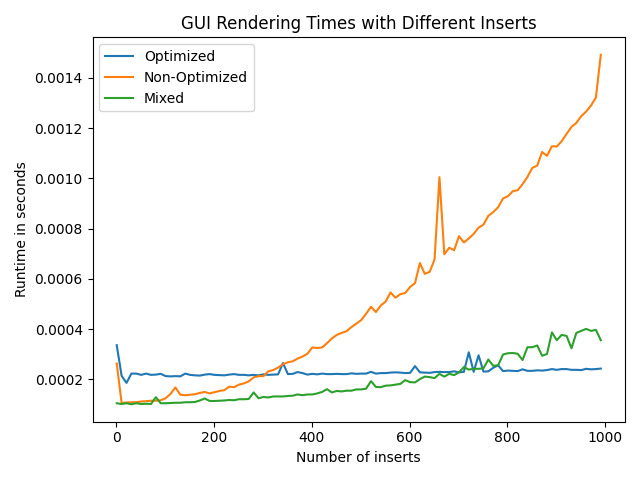
\includegraphics[width=\textwidth]{./images/Profiler-Render-Metric-Size1.jpg}
    \label{fig:renderMetric}
\end{subfigure}
\hfill
\begin{subfigure}[b]{0.3\textwidth}
    \centering
    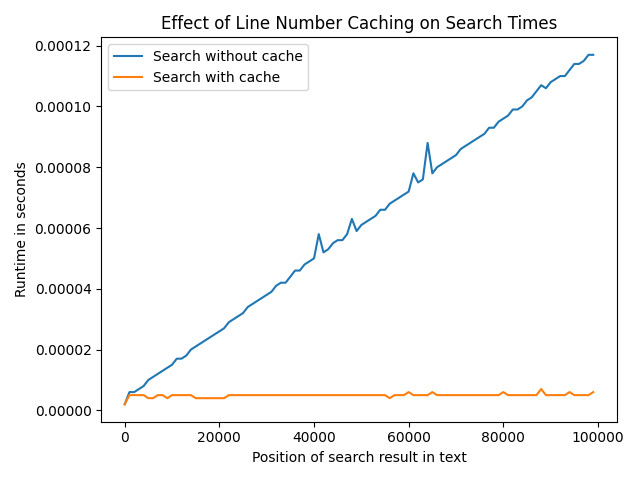
\includegraphics[width=\textwidth]{./images/Profiler-Find-Caching.jpg}
    \label{fig:findMetric}
\end{subfigure}
\hfill
\begin{subfigure}[b]{0.3\textwidth}
    \centering
    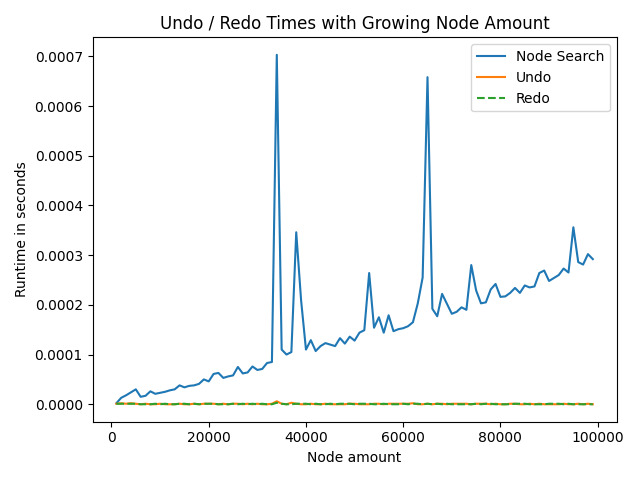
\includegraphics[width=\textwidth]{./images/Profiler-Undo-Redo.jpg}
    \label{fig:undoMetric}
\end{subfigure}
\label{fig:codeStructure}
\end{figure}

%GUI
\begin{figure}[h]
    \centering
    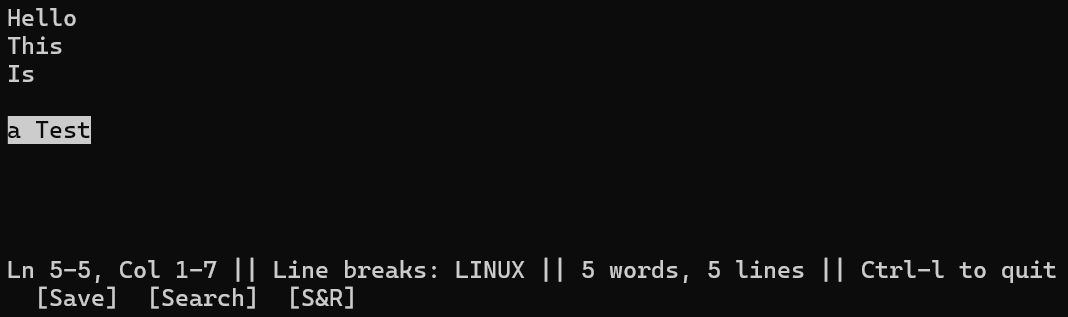
\includegraphics[width=1.0\linewidth]{figures/results_terminal.png}
    \caption{GUI of our text editor running on WSL}
    \label{fig:GUIterminal}            
\end{figure}
\noindent
Above you can see our GUI. From the top left you can see 5 lines written, one of the blank.
\\'a Test' is marked and can be use to copy/paste or delete this section.
Ln 5-5 means marked are rows from 5 to 5, same for Col but column 1 to 7.
'Line breaks: LINUX' means that the current line break style used is LINUX ($\backslash$n). It also supports MSDOS ($\backslash$r$\backslash$n) and MAC ($\backslash$r).
\\Next to it you also have total line and total word count and to the right is the short-cut to exit the editor.
At the very bottom are buttons that you can press to use them. S\&R means search and replace.
\\All aspetcs of our GUI will be shown in this video \cite{demo}, as some of these things are impractical to show on a picture.
    \section{Discussion}\label{sec:discussion}
% Discuss the achieved results (good and bad), their limitation(s) and significance for solving the problem.
    \section{Conclusion}\label{sec:conclusion}
% Summarize what has been achieved, what is left open from your initial plan, and how your solution could
% be further developed/improved through future work.
    \section{Lessons Learned}\label{sec:lessons}
% What did you learn during the project? Which skills did you acquire? What did you learn about
% yourself and your role in a software development team?

    %% References, add them to references.bib
    \bibliographystyle{ieeetr}
    \bibliography{references}
    \addcontentsline{toc}{section}{References}

    \clearpage
    \appendix
     % Redefine the section command for appendices to include the appendix label and number in the title
    \let\oldsection\section
    \renewcommand{\section}[1]{
      % Increment the chapter counter right away
      \refstepcounter{section}
      % Manually format the chapter title to include the appendix label on a separate line and potentially in a smaller font
      % Adjust this line to match your template's specific styling needs
      \oldsection*{{\appendixname\ \thesection}: #1}
      % Add the custom TOC entry with the correctly incremented chapter number
      \addcontentsline{toc}{section}{\appendixname\ \thesection: #1}
    }
    \section{Plots}\label{sec:appendixA}



\section{Materials}\label{sec:appendixB}
\subsection{Software Requirements}\label{SwReq}
Requrements we set ourselves at the initial project submission:
\begin{itemize}
    \item custom data structure
    \item possibility to open files
    \item utf8 support
    \item line break styles
    \item move cursor
    \item clickable buttons
    \item selectable text
    \item edit text
    \item special functions: find, replace
    \item copy ,paste
    \item handle different line break standards
    \item word count statistic
    \item line break type statistic
\end{itemize}
Additional requirements we managed to do:
\begin{itemize}
    \item cursor position statistic
    \item line statistic 
    \item replace all occurences
\end{itemize}
    \clearpage
\section{Declaration of Independent Authorship}\label{sec:integrity}

Copy text from \url{https://dmi.unibas.ch/fileadmin/user_upload/dmi/Studium/Computer_Science/Diverses/Verwendung_AI/2025-02-17_Eigenstaendigkeitserklaerung_Declaration-of-Independent-Authorship_DE_EN_neu.pdf}


\noindent\Large{\textbf{And sign it (all authors!)}}

\begin{figure}[b]
    \centering
    % trim = <left> <bottom> <right> <top>
    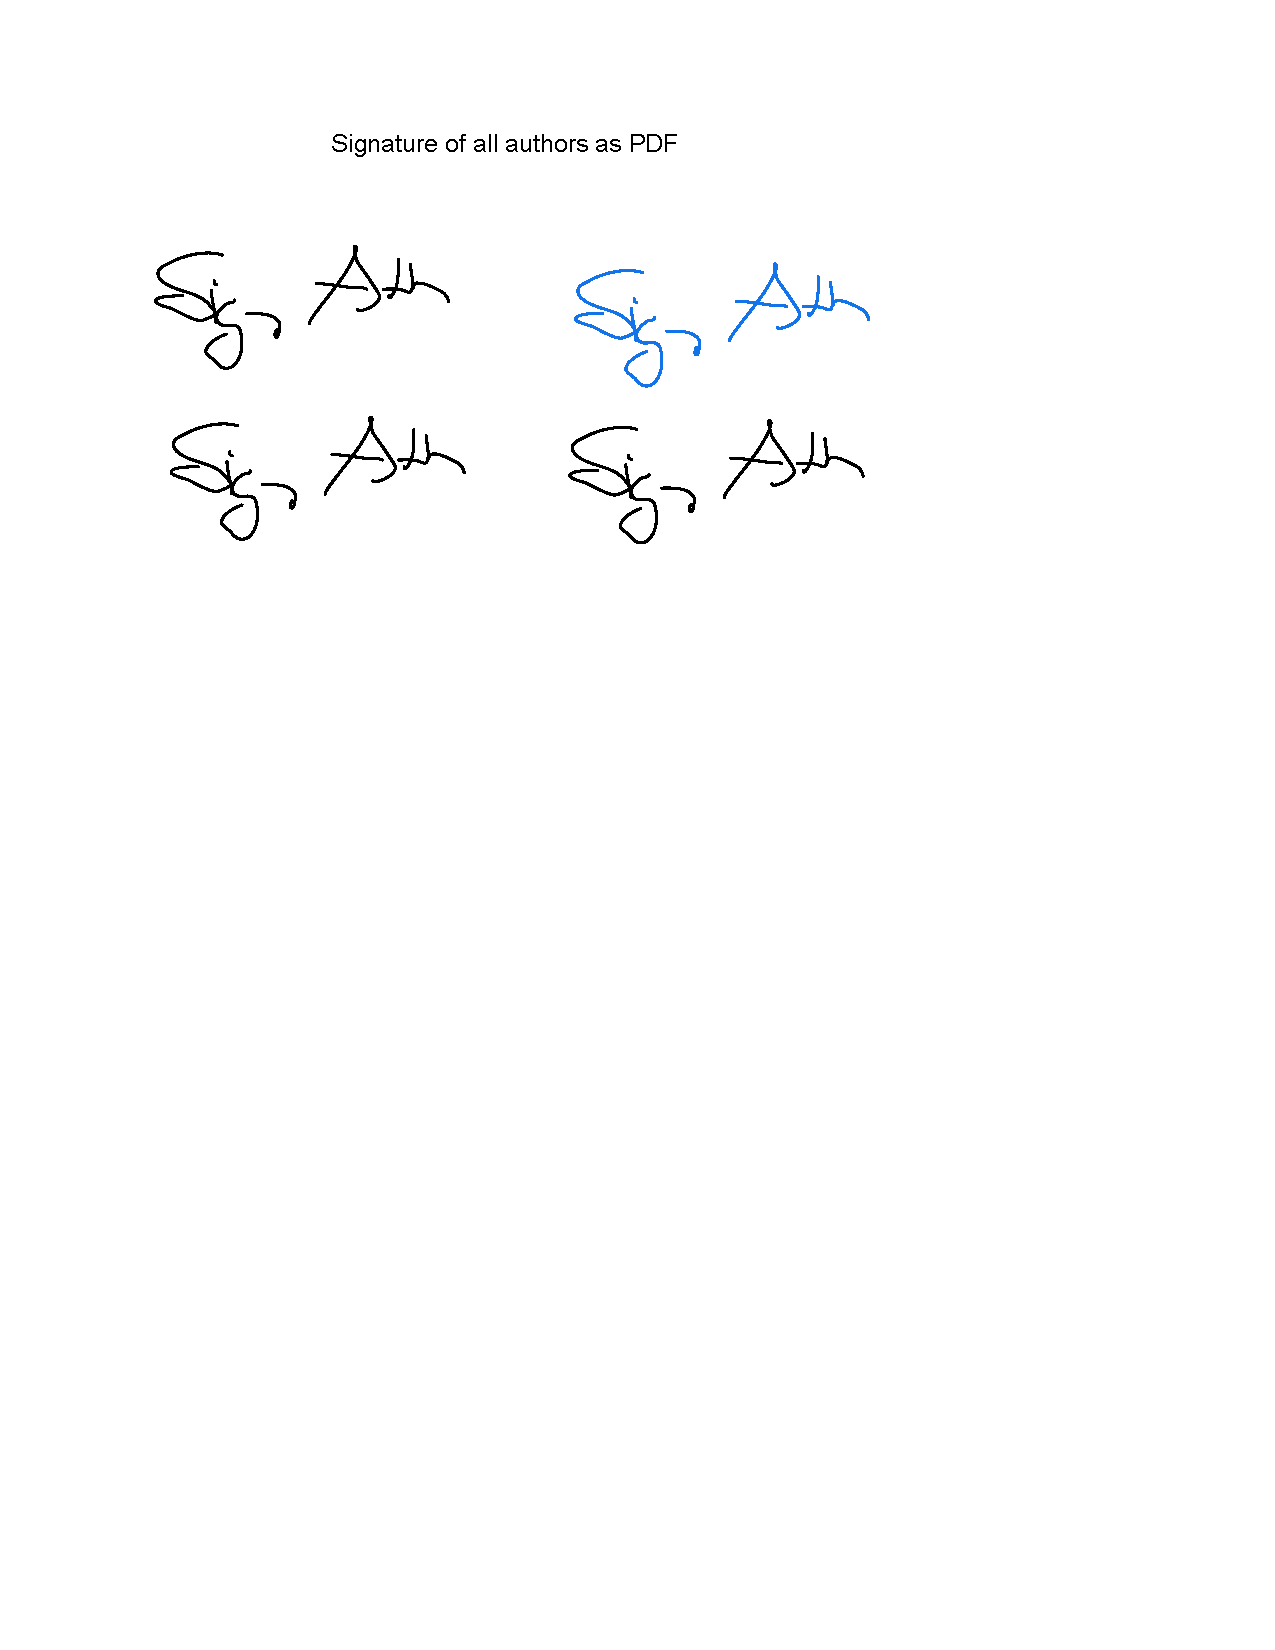
\includegraphics[width=1\textwidth, trim=0pt 500pt 0pt 50pt, clip]{images/example.pdf}
\end{figure}



\end{document}
